%%%%%%%%%%%%%%%%%%%%%%%%%%%%%%%%%%%%%%%%%%%%%%%%%%%%%%%%
% Doctoral Thesis                                      %
% Original authors : Ngoc-Tu Nguyen (Ph.D)             %
% Department of Electronic Engineering                 %
% National Kaohsiung University of Applied Sciences    %
% Email : kuastu2011@gmail.com                         %
% Website : http://203.64.101.229/ngoctu/              %
% Version 1.0 (15/11/2015)                             %
%%%%%%%%%%%%%%%%%%%%%%%%%%%%%%%%%%%%%%%%%%%%%%%%%%%%%%%%

%----------------------------------------------------------------------------------------
%	PACKAGES AND OTHER DOCUMENT CONFIGURATIONS
%----------------------------------------------------------------------------------------

\documentclass[oneside,
12pt, % The default document font size, options: 10pt, 11pt, 12pt
%oneside, % Two side (alternating margins) for binding by default, uncomment to switch to one side
english, % ngerman for German
onehalfspacing, % Single line spacing, alternatives: onehalfspacing or doublespacing
%draft, % Uncomment to enable draft mode (no pictures, no links, overfull hboxes indicated)
%nolistspacing, % If the document is onehalfspacing or doublespacing, uncomment this to set spacing in lists to single
%liststotoc, % Uncomment to add the list of figures/tables/etc to the table of contents
%toctotoc, % Uncomment to add the main table of contents to the table of contents
%parskip, % Uncomment to add space between paragraphs
]{MastersDoctoralThesis} % The class file specifying the document structure

\usepackage{CJKutf8}
\usepackage[utf8]{inputenc} % Required for inputting international characters
\usepackage[T1]{fontenc} % Output font encoding for international characters
\usepackage{palatino} % Use the Palatino font by default
\usepackage{amsopn}
\usepackage[printwatermark]{xwatermark}
\usepackage{transparent}
\usepackage{xcolor}



%\usepackage[backend=bibtex,style=authoryear,natbib=true]{biblatex} % User the bibtex backend with the authoryear citation style (which resembles APA)

%\addbibresource{example.bib} % The filename of the bibliography

\usepackage[autostyle=true]{csquotes} % Required to generate language-dependent quotes in the bibliography


%\newwatermark[pages=1-112,fontfamily=bch,color=gray!100,scale=4,xpos=4,ypos=20]{\includegraphics[width=2cm]{logos/logo.pdf}}
%\newwatermark[allpages,color=red!50,angle=45,scale=3,xpos=-15,ypos=20]{DRAFT VERSION}


%----------------------------------------------------------------------------------------
%	THESIS INFORMATION
%----------------------------------------------------------------------------------------

\thesistitle{論文題目寫在這} % Your thesis title, this is used in the title and abstract, print it elsewhere with \ttitle
\supervisor{謝慶發 教授} % Your supervisor's name, this is used in the title page, print it elsewhere with \supname
\examiner{} % Your examiner's name, this is not currently used anywhere in the template, print it elsewhere with \examname
\degree{碩士} % Your degree name, this is used in the title page and abstract, print it elsewhere with \degreename
\author{郭育豪} % Your name, this is used in the title page and abstract, print it elsewhere with \authorname
\addresses{} % Your address, this is not currently used anywhere in the template, print it elsewhere with \addressname

\subject{電子工程系} % Your subject area, this is not currently used anywhere in the template, print it elsewhere with \subjectname
\keywords{} % Keywords for your thesis, this is not currently used anywhere in the template, print it elsewhere with \keywordnames
\university{國立高雄應用科技大學} % Your university's name and URL, this is used in the title page and abstract, print it elsewhere with \univname
\department{電子工程系} % Your department's name and URL, this is used in the title page and abstract, print it elsewhere with \deptname
\group{Wireless Networking and Distributed Computing Lab} % Your research group's name and URL, this is used in the title page, print it elsewhere with \groupname
%\faculty{\href{http://faculty.university.com}{Faculty Name}} % Your faculty's name and URL, this is used in the title page and abstract, print it elsewhere with \facname

\hypersetup{pdftitle=\ttitle} % Set the PDF's title to your title
\hypersetup{pdfauthor=\authorname} % Set the PDF's author to your name
\hypersetup{pdfkeywords=\keywordnames} % Set the PDF's keywords to your keywords 

\begin{document}
\begin{CJK}{UTF8}{bkai}

\CJKindent
\newcommand{\n}{\mbox{\qquad}}

\newtheorem{proper}{Property}%[theorem]

\frontmatter % Use roman page numbering style (i, ii, iii, iv...) for the pre-content pages
\pagestyle{plain} % Default to the plain heading style until the thesis style is called for the body content

    %----------------------------------------------------------------------------------------
%	書名頁
%----------------------------------------------------------------------------------------

\begin{titlepage}
\vspace*{1mm}

\begin{center}

{\LARGE\bfseries  \titletw}\\
\vspace{15mm}
{\LARGE  \titleen}
\vspace{15mm}

{\large\bfseries{研究生:}\large\authortwname\\
\large\bfseries{指導教授:}\large\supervisortwname}

\vspace{15mm}
{\Large\bfseries{\schooltwname}\\
\vspace{4.5mm}
\Large\bfseries{\depttwname{\degreetw 班}}\\
\vspace{4.5mm}
\Large\bfseries \degreetw 論文}\\
\vspace{10mm}

\vspace{4.5mm}
A Thesis Submitted to \deptenname\\
\schoolenname\\
in Partial Fulfillment of the Requirements\\
for the Degree of \degreeen \,of Engineering\\
in \majortwname

\vspace{15mm}
\dateen\\
\schoolenlocation

\vspace{10mm}
\schoolenoldname \,is the predecessor of
National Kaohsiung University of
Science and Technology (renamed on Feb. 1, 2018)

\vspace{10mm}
% {\large\bfseries{\dateROC}}
\fontsize{14pt}{0pt}{\bfseries{\dateROC }}

\end{center}

\end{titlepage} 
    \cleardoublepage
    \newwatermark[allpages,fontfamily=bch,color=gray!100,scale=4,xpos=4,ypos=20]{\transparent{0.4}\includegraphics[width=1.25cm]{Figures/Logos/LOGO.jpg}}
    %%----------------------------------------------------------------------------------------
%	DECLARATION 宣告 PAGE
%----------------------------------------------------------------------------------------

\begin{declaration}

\noindent I, \href{http://203.64.101.229/ngoctu}{\authorname}, declare that the dissertation is the result of \enquote{\ttitle} my own work. This work was done wholly under period time of Ph.D study at \univname. 

\bigskip

This work is original, except where marked by explicit reference in the thesis, and no part of this thesis has previously been submitted for a degree or other qualification at any other University.

\bigskip

Any views expressed in the thesis are those of the author and in no way represent
those of the \univname. I have acknowledged all main sources of help. \\

\bigskip
\vspace{11mm}
\noindent SIGNED:\\
\rule[0.5em]{25em}{0.5pt} % This prints a line for the signature

\noindent DATE: \today\\
\rule[0.5em]{25em}{0.5pt} % This prints a line to write the date
\end{declaration}

 \addchaptertocentry{\authorshipname}
    %\renewcommand{\abstractname}{摘要}
\begin{cntabstract}
\n隨著目前科技越來越進步,也使得人們的生活越來越便捷... 剩下的 交給你了!

\hbox{}
\it{關鍵詞:人工智慧、物聯網}
\end{cntabstract}

\addchaptertocentry{\abstractname}

\thesistitle{English thesis name}
\supervisor{Chin-Fa Hsieh Ph.D.}
\degree{Master}
\author{Shio-Min Wang}
\subject{Department of Electronic Engineering}
\university{National Kaohsiung University of Science and Technology}
\department{Department of Electronic Engineering}
\group{AIoR Lab}

\renewcommand{\abstractname}{Abstract}
\begin{engabstract}

With the advancement of science and technology, people's lives are becoming more and more convenient ... the rest is left to you

\hbox{}
\it{Keywords: Artificial intelligence,Internet of Things}
\end{engabstract} \addchaptertocentry{\abstractname} % Add the abstract to the table of contents
    %\renewcommand{\acknowledgementname}{誌謝}
\begin{acknowledgements}

謝謝天~ 謝謝地~ 謝謝蜂蜜檸檬!
\end{acknowledgements}  \addchaptertocentry{\acknowledgementname}
    %%----------------------------------------------------------------------------------------
%	publication 出版物 PAGE
%----------------------------------------------------------------------------------------

\begin{publication}

\begin{center}
{\color{red}The first author is my advisor, Dr. Bing-Hong Liu. It's required to Ph.D candidate for conditional graduation in my department.}
\end{center}

\noindent There are all publications in period of Ph.d study :

\begin{itemize}
\item {\color{blue}Journal Publications}.
    \begin{enumerate}
        \item Bing-Hong Liu, \textbf{Ngoc-Tu Nguyen}, Van-Trung Pham, and Yu-Huan Yeh
		"A Maximum-Weight-Independent-Set-Based Algorithm for Reader-Coverage Collision Avoidance Arrangement in RFID Networks", \emph{IEEE Sensors Journal}, (Accepted), Ranking (Q2) - Impact Factor (1.762).

        \item Bing-Hong Liu, \textbf{Ngoc-Tu Nguyen}, Van-Trung Pham, and Wei-Sheng Wang
		"Constrained node-weighted Steiner tree based algorithms for constructing a wireless
		sensor network to cover maximum weighted critical square grids",
		\emph{Computer Communications}, (Accepted), Ranking (Q1) - Impact Factor (1.695).

        \item Bing-Hong Liu, \textbf{Ngoc-Tu Nguyen}, Van-Trung Pham, and Yue-Xian Lin
		"Novel Methods for Energy Charging and Data Collection in Wireless Rechargeable Sensor Networks",
		\emph{International Journal of Communication Systems}, (Accepted), Ranking (Q2) - Impact Factor (1.106).

        \item Bing-Hong Liu, \textbf{Ngoc-Tu Nguyen}, Van-Trung Pham, and Ting-Yan Liou
		"An Efficient Minimum-Latency Collision-Free Scheduling Algorithm for Data Aggregation in Wireless Sensor Networks",
		\emph{IEEE Transactions on Wireless Communications}, (Under review), Ranking (Q1) - Impact Factor (2.496).

        \item Bing-Hong Liu, Van-Trung Pham, and \textbf{Ngoc-Tu Nguyen}
		"An Efficient Algorithm of Constructing Virtual Backbone Scheduling for Maximizing the Lifetime of Dual-Radio Wireless Sensor Networks", \emph{International Journal of Distributed Sensor Networks}, (Accepted), Ranking (Q4) - Impact Factor (0.665).

        \item Bing-Hong Liu, Van-Trung Pham, \textbf{Ngoc-Tu Nguyen}, and Yi-Sheng Luo
		"On Maximizing the Lifetime for Data Aggregation in Wireless Sensor Networks Using Virtual Data Aggregation Trees",
		\emph{IEEE Sensors Journal}, (Under review), Ranking (Q2) - Impact Factor (1.762).

        \item Bing-Hong Liu, Van-Trung Pham, \textbf{Ngoc-Tu Nguyen}, and Chen-Yong Huang
		"An efficient deployment sensors and scheduling mobile devices algorithm for energy charging and data collection with multiple sink", \emph{IEEE Transactions on Computers}, (Under review), Ranking (Q1) - Impact Factor (1.659).
    \end{enumerate}

\item {\color{blue}Conference Publications}.
    \begin{enumerate}
        \item Bing-Hong Liu, \textbf{Ngoc-Tu Nguyen}, and Van-Trung Pham
		"An Efficient Method for Sweep Coverage With Minimum Mobile Sensor",
		\emph{International Conference on Intelligent Information Hiding and. Multimedia Signal Processing}, (Accepted).

        \item Bing-Hong Liu, \textbf{Ngoc-Tu Nguyen}, and Van-Trung Pham
		"A Dynamic-Range-Based Algorithm for Reader-Tag Collision Avoidance Arrangement in RFID Networks",
		\emph{International Conference on Electronics, Information and Communication}, (Accepted).

        \item Bing-Hong Liu, and Van-Trung Pham, \textbf{Ngoc-Tu Nguyen},
		"A Virtual Backbone Construction Heuristic for Maximizing the Lifetime of Dual-Radio Wireless Sensor Networks",
		\emph{International Conference on Intelligent Information Hiding and. Multimedia Signal Processing}, (Accepted).
    \end{enumerate}


\end{itemize}

\end{publication}

 \addchaptertocentry{\publicationname}
    %\input{Instance/lamtran} \addchaptertocentry{\publicationname}
    \renewcommand{\contentsname}{目錄}
    %\tableofcontents \addchaptertocentry{\contentsname}% Prints the main table of contents
    %\renewcommand{\listfigurename}{圖目錄}
    %\listoffigures \addchaptertocentry{\listfigurename}% Prints the list of figures
    %\renewcommand{\listtablename}{表目錄}
    %\listoftables \addchaptertocentry{\listtablename}% Prints the list of tables

    %%----------------------------------------------------------------------------------------
%	ABBREVIATIONS 縮寫詞
%----------------------------------------------------------------------------------------
\begin{abbreviations}{ll} % Include a list of abbreviations (a table of two columns)

\textbf{KUAS} & National \textbf{K}aohsiung \textbf{U}niversity of \textbf{A}pplied \textbf{S}ciences\\
\textbf{WSN} & \textbf{W}ireless \textbf{S}ensor \textbf{N}etwork\\
\textbf{WRSN} & \textbf{W}ireless \textbf{R}echargeable \textbf{S}ensor \textbf{N}etwork\\
\textbf{RFID} & \textbf{R}adio \textbf{F}requency \textbf{I}dentification\\
\textbf{WCSGC} & \textbf{W}eighted \textbf{C}ritical \textbf{S}quare \textbf{G}rid \textbf{C}overage\\
\textbf{GA} & \textbf{G}reedy \textbf{A}lgorithm\\
\textbf{GBA} & \textbf{G}roup \textbf{B}ased \textbf{A}lgorithm\\
\textbf{PBA} & \textbf{P}rofit \textbf{B}ased \textbf{A}lgorithm\\
\textbf{PERDC} & \textbf{P}eriodic \textbf{E}nergy \textbf{R}eplenishment and \textbf{D}ata \textbf{C}ollection\\
\textbf{TSP} & \textbf{T}raveling \textbf{S}alesman \textbf{P}roblem\\
\textbf{GSBA} & \textbf{G}roup \textbf{C}ell \textbf{B}ased \textbf{A}lgorithm\\
\textbf{DSBA} & \textbf{D}ominating \textbf{S}et \textbf{B}ased \textbf{A}lgorithm\\
\textbf{CIBA} & \textbf{C}ircle \textbf{I}ntersection \textbf{B}ased \textbf{A}lgorithm\\
\textbf{MDSA} & \textbf{M}obile \textbf{D}evice \textbf{S}cheduling \textbf{A}lgorithm\\
\textbf{RCCAA} & \textbf{R}eader \textbf{C}overage \textbf{C}ollision \textbf{A}voidance \textbf{A}rrangement\\
\textbf{RRCCAA} & \textbf{R}educed \textbf{R}eader \textbf{C}overage \textbf{C}ollision \textbf{A}voidance \textbf{A}rrangement\\
\textbf{MWIS} & \textbf{M}aximum \textbf{W}eight \textbf{I}ndependent \textbf{S}et\\
\textbf{MWISBA} & \textbf{M}aximum \textbf{W}eight \textbf{I}ndependent \textbf{S}et \textbf{B}ased \textbf{A}lgorithm\\
\textbf{GDE} & \textbf{G}reedy \textbf{D}istributed \textbf{E}limination\\
\textbf{EGDEA} & \textbf{E}xtended \textbf{G}reedy \textbf{D}istributed \textbf{E}limination \textbf{A}lgorithm\\




\end{abbreviations}  \addchaptertocentry{\abbrevname}
    %\input{Instance/constant}
    %\input{Instance/symbol}

%----------------------------------------------------------------------------------------
%	DEDICATION
%----------------------------------------------------------------------------------------

%\dedicatory{For/Dedicated to/To my\ldots}

%----------------------------------------------------------------------------------------
%	THESIS CONTENT - CHAPTERS
%----------------------------------------------------------------------------------------
    \mainmatter % Begin numeric (1,2,3...) page numbering
    \pagestyle{thesis} % Return the page headers back to the "thesis" style

    % 本文
    \chapter{系統概述} % Main chapter title
\label{chapter1} % For referencing the chapter elsewhere, use \ref{1_Chapter1}
\ifpdf
    \graphicspath{{Figures/chapter1/PNG/}{Figures/chapter1/PDF/}{Figures/chapter1/}}
\else
    \graphicspath{{Figures/chapter1/EPS/}{Figures/chapter1/}}
\fi


\section{主機狀況}\label{1_sec:define}
本機一切正常,並無出現特殊硬體錯誤與問題。

\subsection{硬體配備}\label{1_subsec:WCSGC}

\begin{itemize}
    \item CPU
    \item Memoy
    \item Graphic
    \item Hard Disk
    \item SSD
\end{itemize}

\begin{figure*}
    \centering
    \subfigure[]{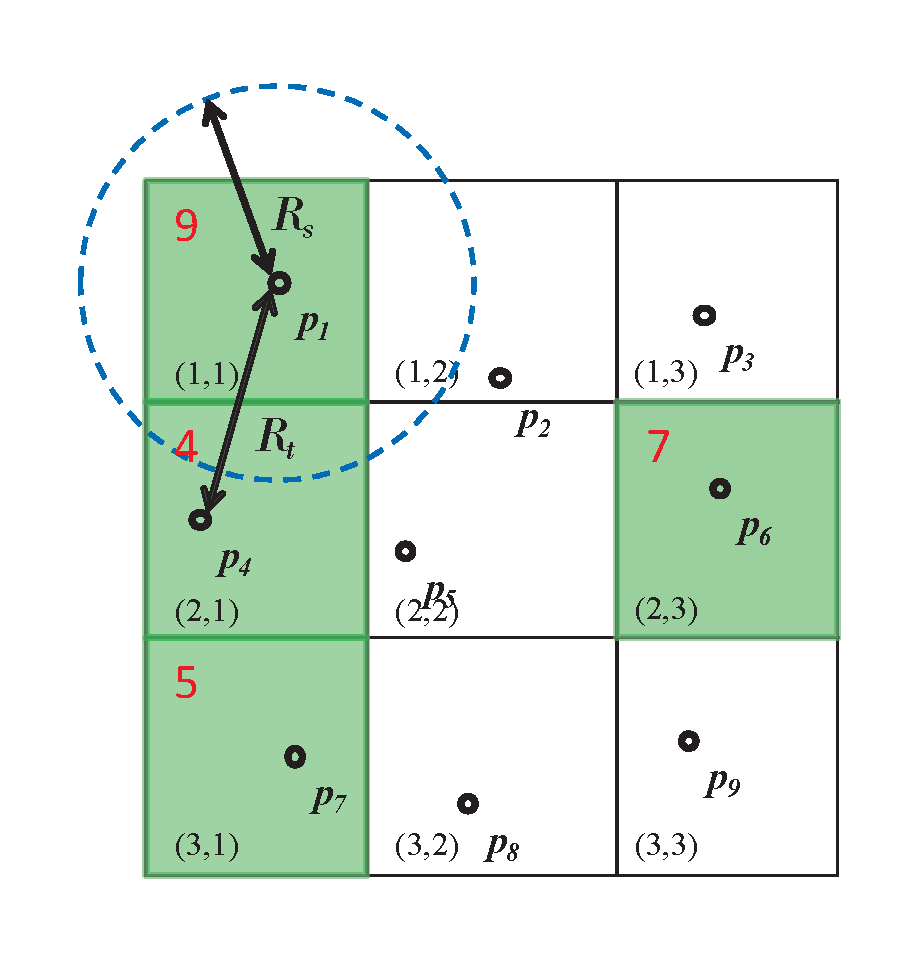
\includegraphics[width=6.5cm]{2a.eps}\label{1_fig_network_model:a}}
    \subfigure[]{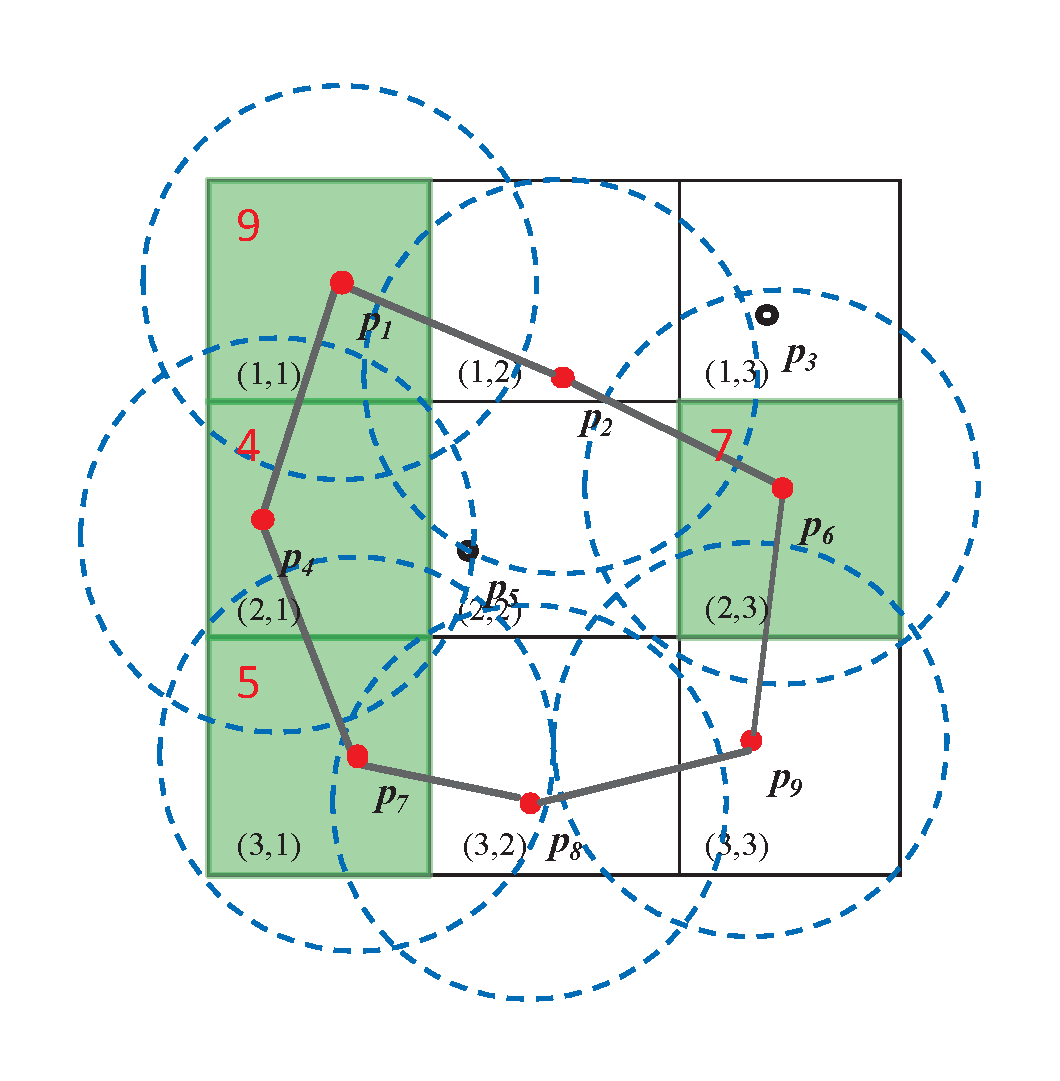
\includegraphics[width=7cm,height=7cm]{2b.eps}\label{1_fig_network_model:b}}
    \caption{Example of the
    weighted-critical-square-grid coverage problem. (a) A sensor field
    divided into $9$ grids of squares with length $\ell$, where
    $R_s=\frac{\sqrt{3}}{2}\ell$, $R_t=\ell$, every grid is labeled with
    a pair of numbers, four critical grids are labeled with $(1,1)$,
    $(2,1)$, $(2,3)$, and $(3,1)$ are shown in green, the weight of each
    critical grid is shown in red, and hollow circles are the points
    that are allowed to deploy sensors. (b) A wireless sensor network
    constructed by $7$ sensors denoted by solid circles, where an edge
    between two sensors represents that the two sensors can communicate
    with each other.} \label{1_fig_network_model}
\end{figure*}



%----------------------------------------------------------------------------------------
%	THESIS CONTENT - APPENDICES
%----------------------------------------------------------------------------------------
%\appendix % Cue to tell LaTeX that the following "chapters" are Appendices

    % Include the appendices of the thesis as separate files from the Appendices folder
    % Uncomment the lines as you write the Appendices

    %\input{Appendices/AppendixA}
    %\input{Appendices/AppendixB}
    %\input{Appendices/AppendixC}

    %----------------------------------------------------------------------------------------
    %	BIBLIOGRAPHY
    %----------------------------------------------------------------------------------------

% \printbibliography[heading=bibintoc]
    %
\renewcommand{\bibname}{參考文獻}
\urlstyle{same}
\printbibliography \addchaptertocentry{\bibname}
%----------------------------------------------------------------------------------------
    %\vspace{1cm}
\begin{flushleft}
\centering
\begin{minipage}{.15\textwidth}
% {\includegraphics[width=1.3in,height=1.7in,clip,keepaspectratio]{ngoc-tu-nguyen.eps}}
\end{minipage}
\hspace{1cm}
\begin{minipage}{.75\textwidth}
\textbf{郭育豪} 2015 年起擔任韌體開發工程師,
2017 年獲得 RedHat 認証系統工程師,
目前是國立高雄科技大學電子工程系碩士班學生也是開源專案 WasmVM 的貢獻者之一,
我的興趣是作業系統與韌體開發,目前正在學習雲端服務與系統的整合。
\end{minipage}
\end{flushleft} 
    % \vspace{1cm}
\begin{flushleft}
\centering
\begin{minipage}{.15\textwidth}
% {\includegraphics[width=1.3in,height=1.7in,clip,keepaspectratio]{ngoc-tu-nguyen.eps}}
\end{minipage}
\hspace{1cm}
\begin{minipage}{.75\textwidth}
\textbf{郭育豪} 2015 年起擔任韌體開發工程師,
2017 年獲得 RedHat 認証系統工程師,
目前是國立高雄科技大學電子工程系碩士班學生也是開源專案 WasmVM 的貢獻者之一,
我的興趣是作業系統與韌體開發,目前正在學習雲端服務與系統的整合。
\end{minipage}
\end{flushleft} 
\newpage
\end{CJK}
\end{document} 